\documentclass[11pt, oneside]{article}   	% use "amsart" instead of "article" for AMSLaTeX format
\usepackage{geometry}                		% See geometry.pdf to learn the layout options. There are lots.
\usepackage{textcomp}
\usepackage[colorlinks=true,urlcolor=blue]{hyperref} 
\geometry{letterpaper}                   		% ... or a4paper or a5paper or ... 
\usepackage[parfill]{parskip}    		% Activate to begin paragraphs with an empty line rather than an indent
\usepackage{graphicx}				% Use pdf, png, jpg, or eps§ with pdflatex; use eps in DVI mode
								% TeX will automatically convert eps --> pdf in pdflatex		
\usepackage{amssymb}
\usepackage{amsmath}
\usepackage{relsize}

\usepackage{tikz}
\usetikzlibrary{arrows,automata}
\usetikzlibrary{positioning}


\tikzset{
    state/.style={
           rectangle,
           rounded corners,
           draw=black, very thick,
           minimum height=2em,
           text centered,
           },
}

\title{CS181 / CSCI E-181 Spring 2014 Final Project}
\author{
  David Wihl\\
  \texttt{davidwihl@gmail.com}
  \and
  Zachary Hendlin\\
  \texttt{zgh@mit.edu} 
}
%\date{}							% Activate to display a given date or no date


\begin{document}
\maketitle

\begingroup
\hypersetup{linkcolor=blue}
\tableofcontents
\endgroup

\section{Introduction}
To gather sufficient data, we allowed the SampleAgent (provided intially in the code) to play ~30 megabytes of ghost training data of games, to get data on feature vectors and associated point values of each.

\section{Classification of Ghosts}
We sought to classify ghosts as \{0, 1, 2, 3, 5\}, where all ghosts in category 5 are dangerous (e.g. induce a reward of -1000 points unless a helpful capsule is consumed first).

We explored two methods for classifying the ghosts on the basis of their features.

First, we explored linear support vector machines using SK-Learn's Stochastic Gradient Descent classifier.
For classifying the category 5 ghosts, this approach was accurate 90.62 percent of the time. Our analysis found that while differences in the rewards associated with eating ghosts not from class 5 did differ by class, the most important thing for us to measure our performance on is the correct classification of dangerous (class 5 ghosts).

<graph here>

We also used logistic regression classification, and achieved somewhat better results, with correct classification of class 5 ghosts 93.25 percent of the time.

We elected to use the logistic regression classification results to predict which class each ghost is in during runtime.

\section{Classification of Capsules and Placebos}
We want to determine which of the pills are helpful capsules and which are placebos. To do this, we first plotted the helpful capsules which we collected using the '-d' data collection function.

Here we determined that capsule feature values were very much clustered into three distinct clusters as shown below.
<show graph>

This suggested that we could either fit Gaussians to these points as part of a generative approach, or apply something like K-means to find the clusters. Because the data were in three dimensions, we opted to use k-means for clustering, and initiated the model with kmeans++.

Because the three clusters were all positively identified, simply assigning a new value at run-time (for a capsule which may be a `good' or `placebo'), we instead used the `score' attribute to evaluate the distance from the centroid the data point would have been assigned to. We are agnostic to which centroid the capsule would be assigned to but we are very sensitive to the score assigned (e.g. the distance from the centroid assignment), with larger distances being worse.

From our positive training data, we found values of $0$ to $-118$ as the `good' range of objective function values. Any value $<-118$ would likely be a placebo capsule.

So at runtime we score each capsule based on its $3\times1$ feature vector and we consider the `best' capsule the one with the maximum objective function value when scored.

\section{Reinforcement Learning}

\section{Rules Engine}
Our next approach was to build a procedural rules engine inspired by a Markov process. In other words, the rules engine did not require any historical data and would simply decide the next action based on the current state of the game.

The other reason for building a rules engine was to better grapple with the game dynamics to see if the model could be significantly simplified. We believe we were successful as the game came down to a straightforward finite state machine. 

We iterated through more than 10 different heuristics. Our average score over 50 games went from a dismal $-7390$ to a reasonable $933$.


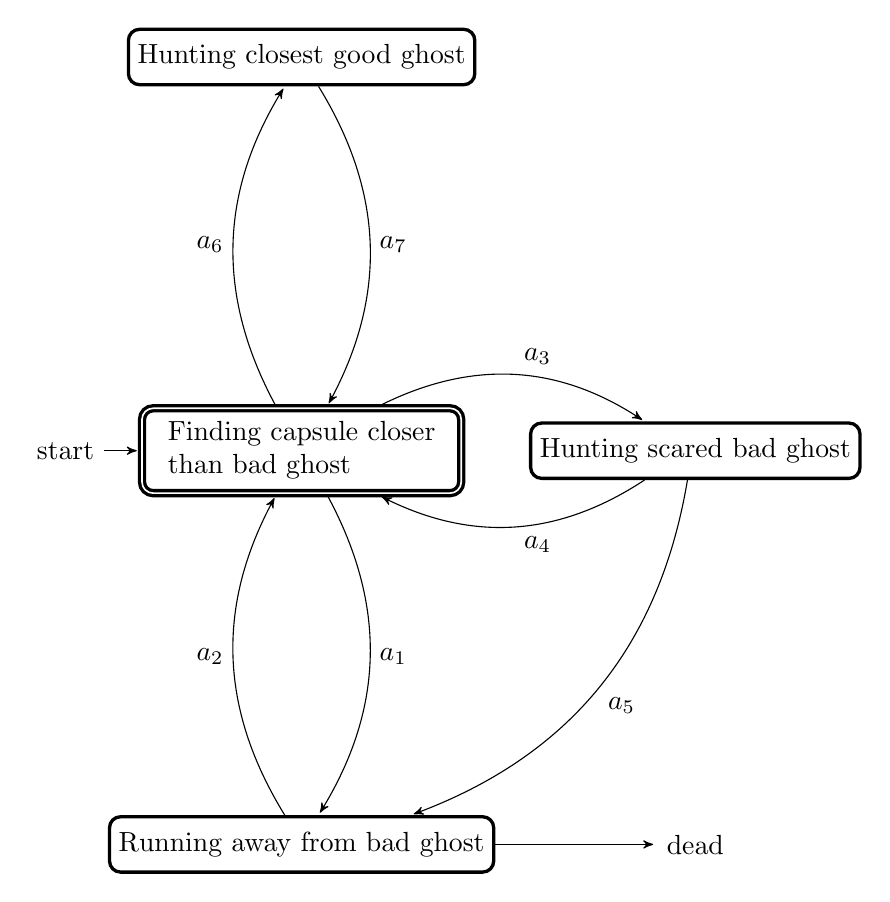
\begin{tikzpicture}[>=stealth',shorten >=1pt,auto,node distance=5cm]
 	\tikzstyle{every state}=[align=center]

	\node[initial,state,accepting] (S1)      
			{
				\begin{tabular}{l}
				Finding capsule closer\\
				than bad ghost
				\end{tabular}
			};
	\node[state]         (S2) [below of=S1]  {Running away from bad ghost};
	\node[state]         (S3) [right of=S1] {Hunting scared bad ghost};
	\node[state]	   (S4) [above of=S1] {Hunting closest good ghost};
	\node[state,draw=none,fill=none]	   (die) [right of=S2] {dead};
	
	\path[->] (S1) edge  [bend left]           node  {$a_3$} (S3);
	\path[->] (S3) edge  [bend left]           node {$a_4$} (S1);
	
	\path[->] (S1) edge  [bend left]           node [align=right] {$a_1$} (S2);
	\path[->] (S2) edge  [bend left]           node {$a_2$} (S1);
	
	\path[->] (S3) edge [bend left]          node {$a_5$} (S2);
	
	\path[->] (S1) edge  [bend left]           node {$a_6$} (S4);
	\path[->] (S4) edge  [bend left]           node {$a_7$} (S1);

	\path[->] (S2) edge node {} (die);
	
\end{tikzpicture}

where:
\begin{description}
	\item[$a_1$] bad ghost closer than good capsule
	\item[$a_2$] good capsule closer than bad ghost
	\item[$a_3$] bad ghost is scared and within range
	\item[$a_4$]bad ghost is out of range
	\item[$a_5$]bad ghost will no longer be scared soon
	\item[$a_6$]no good capsule in range
	\item[$a_7$]good capsule now in range
\end{description}


The Rules engine provided the following advantages:
\begin{description}
	\item[Key Factors]We could distill key factors that would be difficult if not impossible to discover by exploration.
	\item[Latent Factors]One of the key pieces of information was the time remaining before scared bad ghost reverted to normal. We found this by careful examination of the game code. It would have been difficult if not impossible to discover this feature by exploration.
	\item[No history]Since the game changes significantly from one time click to another, a probabilistic model may take time to re-learn the new board. With our ghost and capsule classifiers, we could immediately evaluate the best option from the current board.
	\item[Flexibility]Since only the current state is necessary our rules engine would be flexible enough to handle more dynamics than in the current game. The entire board could resize,  walls could move, capsules could be in motion and the bad ghost could change between time clicks and the rules engine would still find the best course of action.
\end{description}

\section{Parameter Tuning}

\section{Other Methods}
\subsection{Expectimax}
tree would not be deep to merit this. 

\subsection{Alpha-Beta Search}
Russell \& Norvig, pg 166

\subsection{Hidden Markov Model}
 Roland Memisevic
 http://www.iro.umontreal.ca/~memisevr/code/hmm.py

Needed to find a HMM implementation that respected the dependencies of the game cluster. (For example could not use GHMM www.ghmm.org due to a C library dependency)

\section{Conclusion}
A combination of ML and traditional techniques is more powerful than using one set of techniques alone.

\begin{thebibliography}{1}

 \bibitem{item1}\emph{Reinforcement Learning}, Sutton \& Barto, 1998, ISBN-10: 0-262-19398-1
 
  \end{thebibliography}

\end{document}  
